% The document class marks this as a poster, supplying various options that
% control rendering of some standard features (e.g., the title bar).

\documentclass[ % the name of the author
                    author={Luke Murray},
                % the name of the supervisor (preferably including title)
                supervisor={Dr. Simon Hollis},
                % the thesis    title (which cannot be blank)
                     title={Shadow Peer-to-Peer Networks},
                % the thesis subtitle (which can    be blank)
                  subtitle={},
                % the degree programme (from BSc, MEng, MSci, MSc and PhD)
                    degree={MEng},
                % the year of submission
                      year={2013} ]{poster}

\usepackage{epstopdf}
\usepackage{algorithm2e}
\begin{document}

% -----------------------------------------------------------------------------

\begin{frame}{} 

\vfill

\begin{columns}[t]
    \begin{column}{0.900\linewidth}
    \begin{block}{\normalsize Introduction}
    \small Shadow P2P is a network designed to provide a level of anonymity that has never been provided before. On existing networks, it is very hard to tell what a communication is about or who is talking with who. My network aims to provide these anonymity features and it also aims to prevent anyone from being able to tell if a person is participating in the network or not. This is a feature not offered by any other network. This is achieved through the use of several key project components. Among these are: shouts, shout groups, public key hiding and a toroidal network structure.
    \end{block}
    \end{column}
\end{columns}

\vfill

\begin{columns}[t]
    \begin{column}{0.422\linewidth}
    \begin{block}{\normalsize 1. Shouts}
%    \small A shout is essentially a multicast. This is where a message is sent to a known list of IP addresses. In my network, the receiver provides a list of IP addresses, only one of which is the receiver's true IP address. This list is called a 'shout list'. The sender "shouts" by sending a message to every IP address in the shout list whilst also spoofing their own IP address. This anonymises the receiver's IP address amongst those in the shout list and the sender's identity has been removed the message. This method of communication reveals very little about who is talking to who and is the communication primitive that the network depends on.
    \begin{figure}[h]
        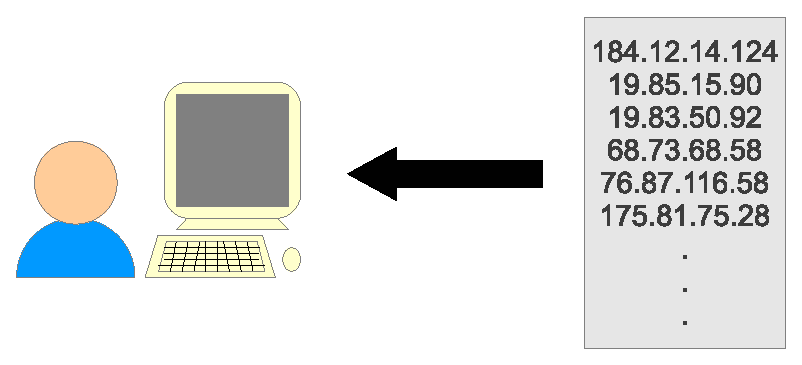
\includegraphics{diagrams/poster_get_list.eps}
        \caption{1. Peer gets the shout list of another peer.}
    \end{figure}
    \begin{figure}[h]
        
\includegraphics{diagrams/poster_spoof_IP.eps}
        \caption{2. Peer sets up IP address spoofing.}
    \end{figure}
    \begin{figure}[h]
        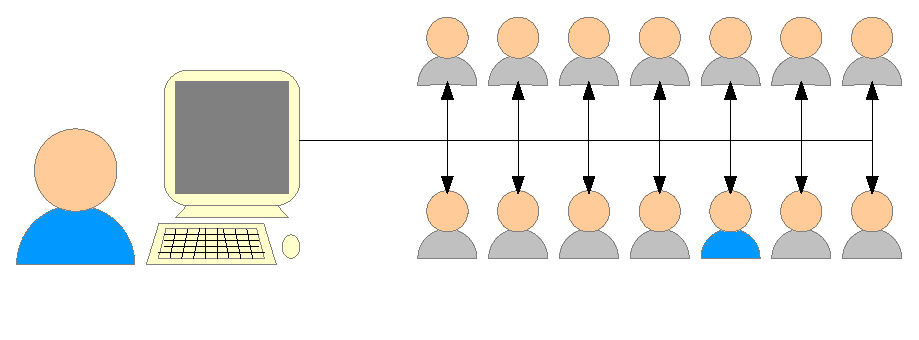
\includegraphics{diagrams/poster_d2.eps}
        \caption{3. Peer sends messages to each IP on the shout list.}
    \end{figure}
%    The communication is unreliable, so how do we make sure the receiver gets the message? How do we prevent a hostile sender from searching the shout list to find the receiver's real IP address? Isn't this method of sending messages not incredibly inefficient?
    \end{block}
    \end{column}

    \begin{column}{0.422\linewidth}
    \begin{block}{\normalsize 2. Shout Groups}
%    \small Shout groups are a defence mechanism against hostile parties searching through the IP addresses on the shout list. A small number of peers work together and create a joint shout list that contains all of their real IP addresses. These peers work together to ensure that they only respond to messages that have been shouted to the entire shout list.
    \begin{figure}[h]
        
\includegraphics{diagrams/poster_search_list.eps}
        \caption{An adversary may attempt to search the shout list for the IP addresses of the peers.}
    \end{figure}
    \begin{figure}[h]
        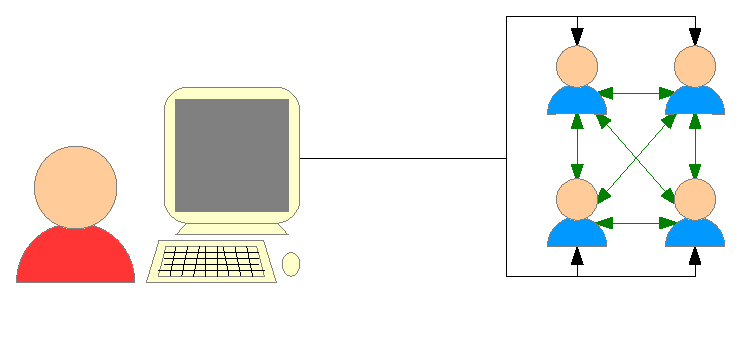
\includegraphics{diagrams/poster_d3.eps}
        \caption{The peers exchange messages to prevent the adversary from doing this.}
    \end{figure}
    \begin{figure}[h]
        \includegraphics{diagrams/poster_getting_old.eps}
        \caption{}
    \end{figure}
%    The peers need to be careful which messages they do or do not respond to; the different search methods used by a hostile sender can reveal information about the peers in the shout group. The aim of the shout group is to minimise the amount of information that a hostile sender can gain about the peers' IP addresses. What if the members of the shout group are hostile? How do the shout group members communicate amongst themselves? How are repeated attacks hindered?
    \end{block}
    \end{column}
\end{columns}

\vfill

\begin{columns}[t]
    \begin{column}{0.422\linewidth}
    \begin{block}{\normalsize 3. Public Key Hiding}
    \small Peers are associated with a public key. This can reveal who is communicating with whom, even with anonymous identities. To prevent this I have invented a method of hiding a public key such that it becomes unrecognisable but such that it can still be used for encryption. In ElGamal, this can be done as follows:
    \begin{figure}[h]
        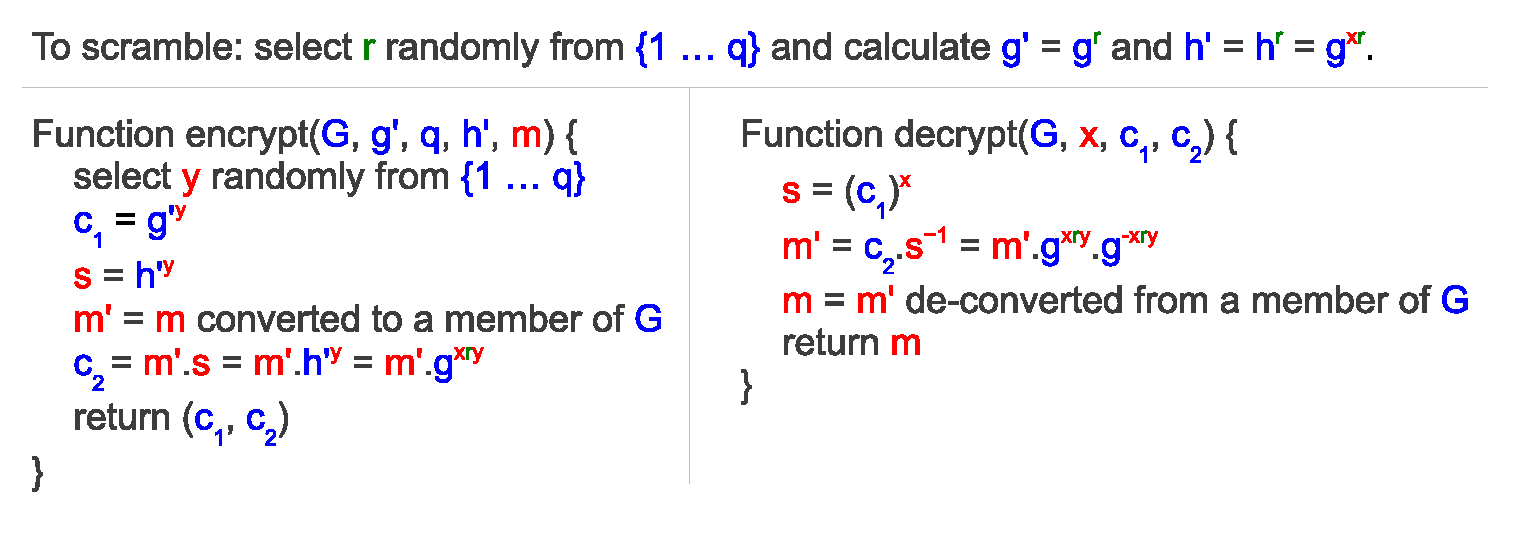
\includegraphics{diagrams/poster_d4.eps}
    \end{figure}    
    This method of public key hiding also works with ECIES (Elliptic Curve Integrated Encryption Scheme).
    \end{block}
    \end{column}
    
    \begin{column}{0.422\linewidth}
    \begin{block}{\normalsize 4. Network Structure}
    \small The network uses a uni-directional toroidal structure through which to deliver packets. This regular structure allows packets to be routed in many different ways making it very difficult to perform traffic analysis. The structure also allows easy dynamic expansion and contraction of the network.
    \begin{figure}[h]
        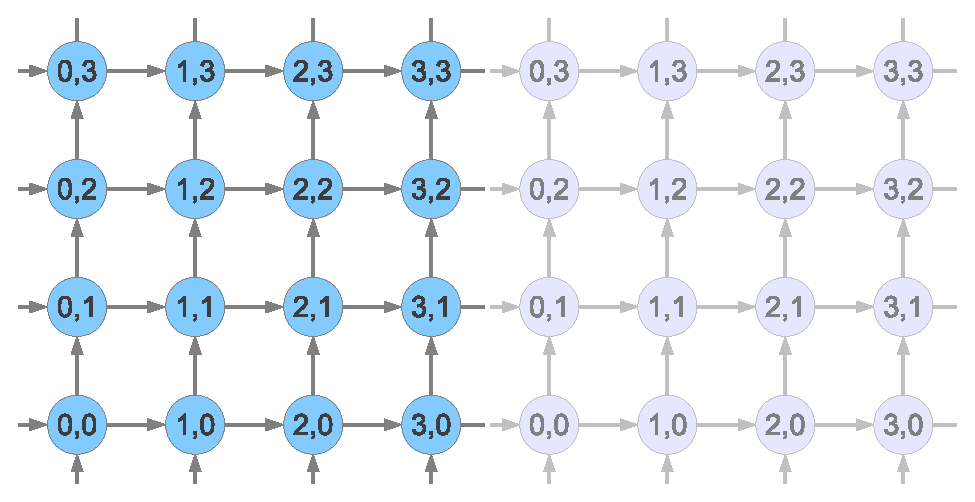
\includegraphics{diagrams/poster_d1.eps}
    \end{figure}
    Nodes transform packets that pass through them so that packets cannot be traced. By using source routing, the sender can be assured that their packets are routed randomly.
    \end{block}
    \end{column}
\end{columns}

\vfill

\end{frame}

% -----------------------------------------------------------------------------

\end{document}



